%============================================================
% CH1 · P3 · PROBLEM 1 — COUNTING ROOMS (CSES 1192)
%============================================================
\subsection{Problem 1.3.1: Counting Rooms}
\problemlabel{1.3.1}{ssec:ch1-counting-rooms}

\problemcard{1.3.1}{Counting Rooms}{CSES 1192}{https://cses.fi/problemset/task/1192}{\exeasy\ (the canonical flood-fill problem)}{Grid as an implicit graph; count connected components with scan + iterative flood fill}

\subsubsection*{1. Problem statement}

You are given the map of a building: $n$ rows and $m$ columns of squares, each either floor (`\texttt{.}') or wall (`\texttt{\#}'). You can walk left, right, up and down through floor squares. Count the \textbf{rooms}: maximal groups of floor squares that are mutually reachable.

\textbf{Constraints:} $1 \le n, m \le 1000$. \quad (The same task appears on LeetCode as ``Number of Islands'', with land \texttt{1} instead of floor.)

\begin{center}
\small
\begin{tabular}{@{}l c@{}}
\toprule
\textbf{Input} & \textbf{Output} \\
\midrule
\texttt{5 8} & \\
\texttt{\#\#\#\#\#\#\#\#} & \\
\texttt{\#..\#...\#} & \\
\texttt{\#\#\#\#.\#.\#} & 3 \\
\texttt{\#..\#...\#} & \\
\texttt{\#\#\#\#\#\#\#\#} & \\
\bottomrule
\end{tabular}
\end{center}

\begin{diagrambox}
\begin{tikzpicture}
    \begin{scope}
        \gIpIIIgrid{wwwwwwww,woowooow,wwwwowow,woowooow,wwwwwwww}
        \foreach \c in {0,...,7} \node[font=\tiny, text=darkgray] at (0.7*\c, 0.5) {\c};
        \foreach \r in {0,...,4} \node[font=\tiny, text=darkgray] at (-0.55, -0.7*\r) {\r};
        \node[font=\small\bfseries] at (2.45,-3.45) {the map};
    \end{scope}
    \begin{scope}[xshift=7.2cm]
        \gIpIIIgrid{wwwwwwww,wAAwBBBw,wwwwBwBw,wCCwBBBw,wwwwwwww}
        \node[font=\small\bfseries] at (2.45,-3.45) {its 3 rooms};
    \end{scope}
\end{tikzpicture}
\figcap{Sample 1. Room A has 2 squares, room B (a ring around the wall at $(2,5)$) has 8, room C has 2. A wall square inside a room does not split it: B is still one room because you can walk around the pillar.}
\end{diagrambox}

\subsubsection*{2. The graph model}

\begin{modelbox}[Graph Model --- Counting Rooms]
\renewcommand{\arraystretch}{1.35}
\begin{tabularx}{\linewidth}{@{}>{\bfseries}l X@{}}
Vertices & the floor squares $(r,c)$; at most $nm = 10^6$ \\
Edges & between two floor squares that share a side (4-neighbourhood); undirected; \textbf{implicit} --- computed from the map, never stored \\
Weights & none \\
Question & the number of \textbf{connected components} \\
Size & $|V| \le 10^6$, $|E| \le 2\cdot10^6$: an $\bigO{|V|+|E|} = \bigO{nm}$ algorithm, about $5\cdot10^6$ simple steps \\
\end{tabularx}
\end{modelbox}

\begin{diagrambox}
\begin{tikzpicture}
    \foreach \r/\c/\s in {1/1/gvA,1/2/gvA, 1/4/gvB,1/5/gvB,1/6/gvB,2/4/gvB,2/6/gvB,3/4/gvB,3/5/gvB,3/6/gvB, 3/1/gvsel,3/2/gvsel}
        \node[\s, minimum size=6.5mm, font=\tiny] (v\r\c) at (1.1*\c, -1.0*\r) {\r,\c};
    \foreach \a/\b in {11/12, 14/15, 15/16, 14/24, 16/26, 24/34, 26/36, 34/35, 35/36, 31/32}
        \draw[ge] (v\a) -- (v\b);
    \node[font=\scriptsize\bfseries, text=primaryblue] at (1.65,-0.45) {A};
    \node[font=\scriptsize\bfseries, text=recursionred] at (5.5,-2.0) {B};
    \node[font=\scriptsize\bfseries, text=softpurple] at (1.65,-3.55) {C};
    \node[note, anchor=west, text width=5.2cm, align=left] at (7.6,-2.0) {12 vertices, 10 edges, 3 components. Component B is a \textbf{cycle} of 8 vertices --- cycles are no problem for a fill, because \texttt{visited} stops it from going round forever.};
\end{tikzpicture}
\figcap{The implicit graph of the sample. Walls have no vertex; the answer is the number of pieces of this graph.}
\end{diagrambox}

\subsubsection*{3. Key observations}

\begin{itemize}[leftmargin=*]
    \item \textbf{A room is a connected component} of the floor graph --- ``you can walk between any two of its squares, and it cannot be extended'' is word for word the definition of a component.
    \item \textbf{Counting components = counting fills.} Scan the map; every floor square that is not yet in a counted room starts a new room, and a fill marks that whole room (Pattern 3 invariant).
    \item \textbf{The grid can be its own \texttt{visited} array}: turning a visited `\texttt{.}' into `\texttt{\#}' never changes the answer, because that room is already counted.
    \item \textbf{Depth trap:} $nm$ reaches $10^6$, and a recursive fill on an open $1000\times1000$ room recurses $10^6$ levels deep. Use an explicit stack.
\end{itemize}

\subsubsection*{4. Approaches}

\begin{bruteforcebox}[Approach 1: Brute Force --- Label Propagation]
\textbf{Idea.} Give every floor square its own id as a label. Repeat sweeps over the map: each square takes the \emph{smallest} label among itself and its floor neighbours. When a sweep changes nothing, every room carries the smallest id of the room; the answer is the number of squares whose label is still their own id. No graph search at all --- just a local rule, repeated.

\begin{lstlisting}[style=cpp]
#include <bits/stdc++.h>
using namespace std;

int main() {
    int n, m;
    cin >> n >> m;
    vector<string> g(n);
    for (auto& row : g) cin >> row;
    vector<int> lab(n * m, -1);
    for (int r = 0; r < n; r++)
        for (int c = 0; c < m; c++)
            if (g[r][c] == '.') lab[r * m + c] = r * m + c;

    const int dr[4] = {-1, 1, 0, 0}, dc[4] = {0, 0, -1, 1};
    bool changed = true;
    while (changed) {                       // one round = one sweep over all cells
        changed = false;
        for (int r = 0; r < n; r++)
            for (int c = 0; c < m; c++) {
                if (g[r][c] != '.') continue;
                for (int d = 0; d < 4; d++) {
                    int nr = r + dr[d], nc = c + dc[d];
                    if (nr < 0 || nr >= n || nc < 0 || nc >= m || g[nr][nc] != '.') continue;
                    if (lab[nr * m + nc] < lab[r * m + c]) {
                        lab[r * m + c] = lab[nr * m + nc];
                        changed = true;
                    }
                }
            }
    }
    int rooms = 0;
    for (int i = 0; i < n * m; i++)
        if (lab[i] == i) rooms++;           // the smallest id of each room survives
    cout << rooms << "\n";
}
\end{lstlisting}

\begin{diagrambox}
\begin{tikzpicture}
    \begin{scope}
        \def\gIpIIIs{0.32}
        \gIpIIIgrid{ooooooooo,wwwwwwwwo,ooooooooo,owwwwwwww,ooooooooo,wwwwwwwwo,ooooooooo,owwwwwwww,ooooooooo}
    \end{scope}
    \node[note, anchor=west, text width=4.6cm, align=left] at (3.3,-1.3) {A ``snake'' room: one long corridor folded back and forth. A small label must travel along the whole corridor, and against the sweep direction it moves only about one square per sweep.};
    \node[font=\scriptsize] at (10.4,-1.3) {
        \begin{tabular}{@{}rr@{}}
        \toprule
        snake $n\times n$ & sweeps \\
        \midrule
        $20\times20$ & 97 \\
        $40\times40$ & 392 \\
        $80\times80$ & 1582 \\
        \bottomrule
        \end{tabular}};
\end{tikzpicture}
\figcap{Measured number of sweeps on snakes: it grows like $nm/4$. For $1000\times1000$ that is about $2.5\cdot10^5$ sweeps of $10^6$ squares each.}
\end{diagrambox}

\begin{complexitybox}
\textbf{Time:} $\bigO{(nm)^2}$ in the worst case (up to $\approx nm/4$ sweeps of $nm$ squares) --- about $2.5\cdot10^{11}$ steps for $1000\times1000$. \textbf{Space:} $\bigO{nm}$. \textbf{Verdict:} \tle{} --- but correct and very easy to trust, so it is our reference on small random maps.
\end{complexitybox}
\end{bruteforcebox}

\begin{algorithmbox}[Approach 2: Scan + Iterative Flood Fill]
\textbf{Idea.} Scan the map; a `\texttt{.}' square starts a new room. Fill that room with an explicit stack, overwriting every reached floor square with `\texttt{\#}' the moment it is pushed. When the scan ends, the counter is the answer.

\begin{lstlisting}[style=cpp]
#include <bits/stdc++.h>
using namespace std;

int main() {
    int n, m;
    scanf("%d %d", &n, &m);
    vector<string> g(n);
    char buf[1005];
    for (int i = 0; i < n; i++) { scanf("%s", buf); g[i] = buf; }

    const int dr[4] = {-1, 1, 0, 0}, dc[4] = {0, 0, -1, 1};
    vector<int> st;                        // explicit stack of cell ids r*m+c
    st.reserve(n * m);
    int rooms = 0;
    for (int r = 0; r < n; r++)
        for (int c = 0; c < m; c++) {
            if (g[r][c] != '.') continue;  // wall, or floor already in a counted room
            rooms++;                       // (r,c) starts a new room
            g[r][c] = '#';                 // mark on PUSH: never pushed twice
            st.push_back(r * m + c);
            while (!st.empty()) {
                int id = st.back(); st.pop_back();
                int cr = id / m, cc = id % m;
                for (int d = 0; d < 4; d++) {
                    int nr = cr + dr[d], nc = cc + dc[d];
                    if (nr < 0 || nr >= n || nc < 0 || nc >= m) continue;  // outside
                    if (g[nr][nc] != '.') continue;                       // wall / seen
                    g[nr][nc] = '#';
                    st.push_back(nr * m + nc);
                }
            }
        }
    printf("%d\n", rooms);
}
\end{lstlisting}

\begin{complexitybox}
\textbf{Time:} $\bigO{nm}$ --- every square is pushed and popped at most once and looks at 4 neighbours. Measured: 0.16\,s for an all-floor $1000\times1000$ map, input included. \textbf{Space:} $\bigO{nm}$ for the map and the stack (the stack never holds more than $nm$ ids). \textbf{Verdict:} \ac{}.
\end{complexitybox}
\end{algorithmbox}

\begin{invariantbox}[Why it is correct]
\textbf{Invariant (between two iterations of the scan):} every floor square of an already counted room has been overwritten with `\texttt{\#}', and no square of an uncounted room has been touched.

\emph{Initially} nothing is counted and nothing is touched. \emph{Step:} when the scan meets a `\texttt{.}' at $(r,c)$, the invariant says its room is uncounted, so \texttt{rooms++} counts it exactly once; the fill then overwrites exactly the squares reachable from $(r,c)$ --- that room and nothing else (Pattern 3, Claim 1). \emph{End:} every floor square was scanned, so every room was met at least once while still untouched, and was counted exactly once. \hfill$\blacksquare$
\end{invariantbox}

\begin{alternativebox}[Approach 3: Alternative Algorithms --- BFS Fill, or DSU]
\textbf{BFS fill.} Replace the stack by a \texttt{queue} and mark on enqueue (template 3 of the theory). Same $\bigO{nm}$, same answer --- checked on 500 random maps against the brute force. BFS is the version you will extend in Chapter 3 to compute distances.

\textbf{DSU preview (Chapter 6).} Start with every floor square as its own room. For each floor square, unite it with its upper and its left floor neighbour; every union of two \emph{different} sets merges two rooms, so \texttt{rooms--}. There is no search order at all --- and it keeps working if floor squares are \emph{added} one at a time, which a fill cannot handle cheaply.
\begin{lstlisting}[style=cpp]
#include <bits/stdc++.h>
using namespace std;

vector<int> par;
int findRoot(int x) {                      // with path halving
    while (par[x] != x) { par[x] = par[par[x]]; x = par[x]; }
    return x;
}
bool unite(int a, int b) {                 // true if two different rooms merged
    a = findRoot(a); b = findRoot(b);
    if (a == b) return false;
    par[a] = b;
    return true;
}

int main() {
    ios::sync_with_stdio(false);
    cin.tie(nullptr);
    int n, m;
    cin >> n >> m;
    vector<string> g(n);
    for (auto& row : g) cin >> row;
    par.resize(n * m);
    for (int i = 0; i < n * m; i++) par[i] = i;
    int rooms = 0;
    for (int r = 0; r < n; r++)
        for (int c = 0; c < m; c++) {
            if (g[r][c] != '.') continue;
            rooms++;                                   // every floor cell starts alone
            if (r > 0 && g[r - 1][c] == '.' && unite(r * m + c, (r - 1) * m + c)) rooms--;
            if (c > 0 && g[r][c - 1] == '.' && unite(r * m + c, r * m + c - 1)) rooms--;
        }
    cout << rooms << "\n";
}
\end{lstlisting}
\end{alternativebox}

\begin{tricksbox}
\begin{itemize}[leftmargin=*]
    \item \textbf{No separate \texttt{visited}:} overwriting the map saves $10^6$ bytes and one comparison per neighbour.
    \item \textbf{Sentinel border:} the sample is surrounded by walls, but that is not promised. If you pad the map yourself with a ring of `\texttt{\#}' (size $(n+2)\times(m+2)$), the four bounds checks disappear from the inner loop.
    \item \textbf{One integer per stack entry} (\texttt{r*m+c}) instead of a \texttt{pair}: half the memory traffic.
    \item \textbf{Fast input:} $10^6$ characters --- read whole rows with \texttt{scanf("\%s")}, or \texttt{cin >> row} after \texttt{sync\_with\_stdio(false)}; never character by character with slow streams.
\end{itemize}
\end{tricksbox}

\subsubsection*{5. Trace}

\begin{tracebox}[{Sample 1 --- the fill of room B (stack, neighbour order up, down, left, right)}]
The scan reaches $(1,1)$ first: room A $=\{(1,1),(1,2)\}$ is filled in two pops. The next `\texttt{.}' is $(1,4)$: \texttt{rooms} becomes 2 and the fill of B starts.

\begin{center}
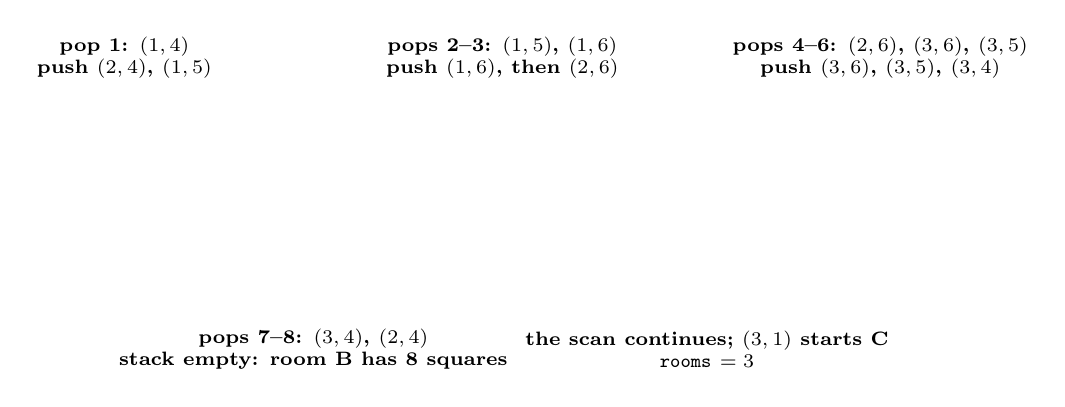
\begin{tikzpicture}
    \def\gIpIIIs{0.5}
    \begin{scope}
        \gIpIIIgrid{wwwwwwww,wAAwxqow,wwwwqwow,woowooow,wwwwwwww}
        \node[font=\scriptsize\bfseries, align=center] at (1.75,-2.6) {pop 1: $(1,4)$\\push $(2,4)$, $(1,5)$};
    \end{scope}
    \begin{scope}[xshift=4.8cm]
        \gIpIIIgrid{wwwwwwww,wAAwkkxw,wwwwqwqw,woowooow,wwwwwwww}
        \node[font=\scriptsize\bfseries, align=center] at (1.75,-2.6) {pops 2--3: $(1,5)$, $(1,6)$\\push $(1,6)$, then $(2,6)$};
    \end{scope}
    \begin{scope}[xshift=9.6cm]
        \gIpIIIgrid{wwwwwwww,wAAwkkkw,wwwwqwkw,woowqxkw,wwwwwwww}
        \node[font=\scriptsize\bfseries, align=center] at (1.75,-2.6) {pops 4--6: $(2,6)$, $(3,6)$, $(3,5)$\\push $(3,6)$, $(3,5)$, $(3,4)$};
    \end{scope}
    \begin{scope}[yshift=-3.7cm, xshift=2.4cm]
        \gIpIIIgrid{wwwwwwww,wAAwBBBw,wwwwBwBw,woowBBBw,wwwwwwww}
        \node[font=\scriptsize\bfseries, align=center] at (1.75,-2.6) {pops 7--8: $(3,4)$, $(2,4)$\\stack empty: room B has 8 squares};
    \end{scope}
    \begin{scope}[yshift=-3.7cm, xshift=7.4cm]
        \gIpIIIgrid{wwwwwwww,wAAwBBBw,wwwwBwBw,wCCwBBBw,wwwwwwww}
        \node[font=\scriptsize\bfseries, align=center] at (1.75,-2.6) {the scan continues; $(3,1)$ starts C\\\texttt{rooms} $= 3$};
    \end{scope}
\end{tikzpicture}
\end{center}
{\small Orange frame = the square just popped; yellow = on the stack (already marked); light blue = popped earlier.}

\begin{center}
\small
\begin{tabular}{@{}clll@{}}
\toprule
\textbf{pop} & \textbf{square} & \textbf{newly pushed} & \textbf{stack after (bottom $\to$ top)} \\
\midrule
1 & $(1,4)$ & $(2,4)$, $(1,5)$ & $(2,4)\ (1,5)$ \\
2 & $(1,5)$ & $(1,6)$ & $(2,4)\ (1,6)$ \\
3 & $(1,6)$ & $(2,6)$ & $(2,4)\ (2,6)$ \\
4 & $(2,6)$ & $(3,6)$ & $(2,4)\ (3,6)$ \\
5 & $(3,6)$ & $(3,5)$ & $(2,4)\ (3,5)$ \\
6 & $(3,5)$ & $(3,4)$ & $(2,4)\ (3,4)$ \\
7 & $(3,4)$ & --- ($(2,4)$ is already marked) & $(2,4)$ \\
8 & $(2,4)$ & --- & empty \\
\bottomrule
\end{tabular}
\end{center}
Pop 7 is where ``mark on push'' pays off: $(2,4)$ is a floor neighbour of $(3,4)$, but it was marked at pop 1, so it is not pushed a second time. The fill went the long way round the ring and closed the cycle without noticing it. Output: \textbf{3}.
\end{tracebox}

\subsubsection*{6. Test suite}

\begin{testbox}
\centering\small
\begin{tabular}{@{}lll@{}}
\toprule
\textbf{Map} & \textbf{Expected} & \textbf{Why} \\
\midrule
the sample & 3 & a room with a pillar is still one room \\
$1\times1$ `\texttt{.}' & 1 & smallest map, no wall border \\
$1\times1$ `\texttt{\#}' & 0 & no floor at all \\
$1000\times1000$ all `\texttt{\#}' & 0 & scan only, no fill \\
$1000\times1000$ all `\texttt{.}' & 1 & one huge room; recursion depth would be $10^6$ \\
$1000\times1000$ checkerboard & 500000 & one-square rooms; diagonal contacts do not count \\
$1000\times1000$ snake & 1 & long corridor; brute force: $\approx 2.5\cdot10^5$ sweeps \\
500 random maps ($\le 8\times8$) & = brute & all four approaches agree \\
\bottomrule
\end{tabular}
\end{testbox}

\subsubsection*{7. Common mistakes}

\begin{warningbox}[{Mistake 1 --- recursive fill on a $1000\times1000$ map}]
\begin{lstlisting}[style=snippet]
void dfs(int r, int c) {                      // depth up to n*m = 10^6
    if (r < 0 || r >= n || c < 0 || c >= m || g[r][c] != '.') return;
    g[r][c] = '#';
    dfs(r - 1, c); dfs(r + 1, c); dfs(r, c - 1); dfs(r, c + 1);
}
\end{lstlisting}
Correct on the sample (maximum depth 8), but on an all-floor $1000\times1000$ map the depth is $10^6$ and the program crashes with the usual stack (we ran it). Use the explicit stack of Approach 2.
\end{warningbox}

\begin{warningbox}[Mistake 2 --- counting squares instead of fills]
``Number of rooms'' counts \emph{fills started}, not squares filled. Put \texttt{rooms++} next to the start of a fill, outside the \texttt{while} loop.
\end{warningbox}

\begin{warningbox}[Mistake 3 --- slow character-by-character input]
\texttt{cin >> ch} for $10^6$ characters on synchronised streams can cost more than the whole algorithm. Read a row at a time.
\end{warningbox}

\begin{warningbox}[Mistake 4 --- adding diagonal neighbours]
The statement says left, right, up, down. With 8 directions the checkerboard test gives 1 instead of 500000.
\begin{center}
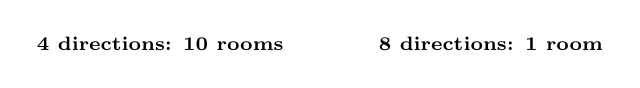
\begin{tikzpicture}
    \def\gIpIIIs{0.45}
    \begin{scope}
        \gIpIIIgrid{awbwc,wdwew,fwawb,wcwdw}
        \node[font=\scriptsize\bfseries] at (0.9,-2.15) {4 directions: 10 rooms};
    \end{scope}
    \begin{scope}[xshift=4.2cm]
        \gIpIIIgrid{awawa,wawaw,awawa,wawaw}
        \node[font=\scriptsize\bfseries] at (0.9,-2.15) {8 directions: 1 room};
    \end{scope}
\end{tikzpicture}
\end{center}
\end{warningbox}

\subsubsection*{8. Takeaways}

\begin{itemize}[leftmargin=*]
    \item Squares = vertices, shared sides = edges; rooms = connected components.
    \item Number of components = number of fills started by the row-major scan.
    \item Mark on push, and let the map be its own \texttt{visited} array.
    \item For $nm$ up to $10^6$: explicit stack or queue, not recursion.
\end{itemize}

\begin{variantsbox}
\variant{Eight directions}{\varnone}
  {squares touching at a corner also belong to the same room.}
  {vertices unchanged; edges also join diagonal neighbours (up to 8 per square).}
  {use the 8-entry direction arrays; everything else is identical, still $\bigO{nm}$.}
\variant{Volume of the biggest lake}{\varin{https://codeforces.com/problemset/problem/1829/E}}
  {cells carry depths; find the component with the largest \emph{sum} of depths.}
  {vertices = cells with depth $> 0$; same 4-neighbour edges.}
  {the fill adds up the values it reaches; answer = the largest sum (Exercise E3.3).}
\variant{Sub-islands}{\varin{https://leetcode.com/problems/count-sub-islands/}}
  {count the islands of grid 2 whose every cell is also land in grid 1.}
  {components of grid 2; a component is ``good'' if all its vertices are land in grid 1.}
  {fill each island of grid 2 completely, AND-ing a flag over its cells; count the good ones (Exercise E3.4).}
\variant{Rooms away from the outside}{\varnone}
  {count only rooms that contain no square of the outer border.}
  {same graph; a component is ``closed'' if none of its vertices lies on row $0$, row $n{-}1$, column $0$ or column $m{-}1$.}
  {first fill from every border floor square and discard those rooms, then count the remaining fills (Chapter 4 studies this ``fill from the border'' idea).}
\variant{Walls broken one by one}{\varnone}
  {after each of $q$ updates ``square $(r,c)$ becomes floor'', print the number of rooms.}
  {the graph only gains vertices and edges.}
  {DSU: a new floor square adds 1 room, every union with a different neighbouring room subtracts 1 (Chapter 6).}
\end{variantsbox}
